\documentclass[border=10pt]{standalone}
\usepackage{tikz}
\usetikzlibrary{positioning,arrows.meta,calc,fit,patterns}

\begin{document}
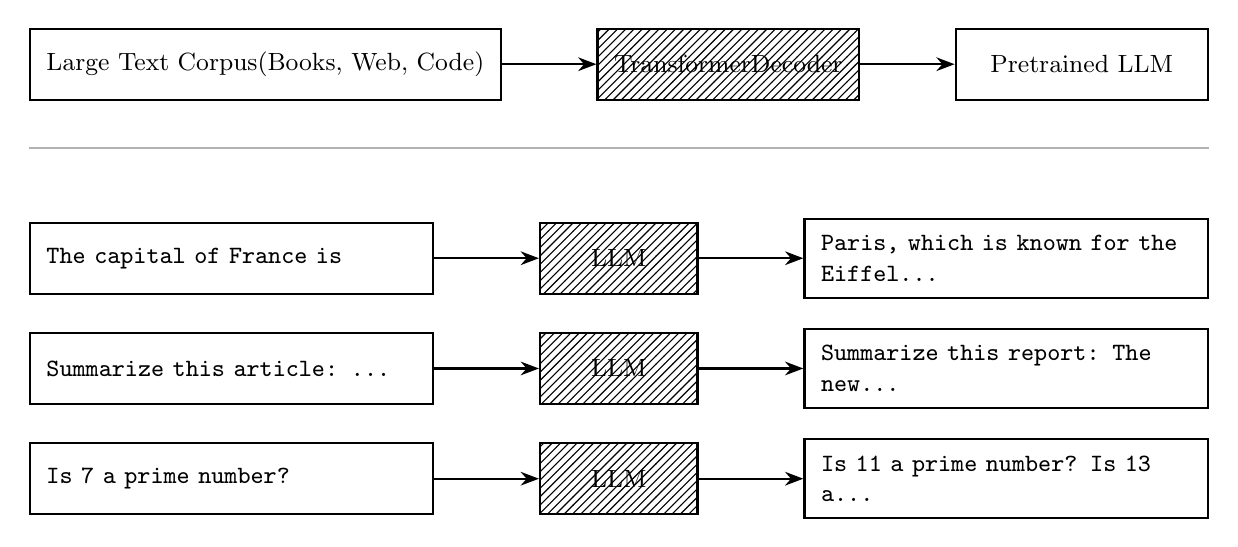
\begin{tikzpicture}[
    >=Stealth,
    every node/.style={font=\small},
    box/.style={draw, thick, minimum height=0.9cm, inner sep=6pt, text centered},
    inputbox/.style={box, fill=white, align=left},
    outputbox/.style={box, fill=white, align=left},
    modelbox/.style={box, pattern=north east lines, minimum width=2.0cm, minimum height=0.9cm},
    flowbox/.style={box, fill=white, minimum width=3.2cm},
    flowarrow/.style={->, thick, black},
]

% ---- Top: Process Flow ----
\node[flowbox] (corpus) {Large Text Corpus\\(Books, Web, Code)};
\node[modelbox, right=1.2cm of corpus] (transformer) {Transformer\\Decoder};
\node[flowbox, right=1.2cm of transformer] (pretrained) {Pretrained LLM};

\draw[flowarrow] (corpus) -- (transformer);
\draw[flowarrow] (transformer) -- (pretrained);

% ---- Divider ----
\draw[thick, black!30] ([yshift=-0.6cm]corpus.south west) -- ([yshift=-0.6cm]pretrained.south east);

% ---- Bottom: Example I/O (centered, equal widths) ----
% Center point of the full figure width
\coordinate (figcenter) at ($(corpus.west)!0.5!(pretrained.east)$);

\coordinate (row1) at ([yshift=-2.0cm]transformer.south);
\coordinate (row2) at ([yshift=-1.4cm]row1);
\coordinate (row3) at ([yshift=-1.4cm]row2);

% Place LLM boxes at the true center of the figure
\node[modelbox, minimum width=2.0cm] (m1) at (figcenter |- row1) {LLM};
\node[modelbox, minimum width=2.0cm] (m2) at (figcenter |- row2) {LLM};
\node[modelbox, minimum width=2.0cm] (m3) at (figcenter |- row3) {LLM};

% Row 1
\node[inputbox, text width=4.7cm, anchor=west] (in1) at (corpus.west |- row1) {\texttt{The capital of France is}};
\node[outputbox, text width=4.7cm, anchor=east] (out1) at (pretrained.east |- row1) {\texttt{Paris, which is known for the Eiffel...}};
\draw[flowarrow] (in1) -- (m1);
\draw[flowarrow] (m1) -- (out1);

% Row 2
\node[inputbox, text width=4.7cm, anchor=west] (in2) at (corpus.west |- row2) {\texttt{Summarize this article: ...}};
\node[outputbox, text width=4.7cm, anchor=east] (out2) at (pretrained.east |- row2) {\texttt{Summarize this report: The new...}};
\draw[flowarrow] (in2) -- (m2);
\draw[flowarrow] (m2) -- (out2);

% Row 3
\node[inputbox, text width=4.7cm, anchor=west] (in3) at (corpus.west |- row3) {\texttt{Is 7 a prime number?}};
\node[outputbox, text width=4.7cm, anchor=east] (out3) at (pretrained.east |- row3) {\texttt{Is 11 a prime number? Is 13 a...}};
\draw[flowarrow] (in3) -- (m3);
\draw[flowarrow] (m3) -- (out3);

\end{tikzpicture}
\end{document}
